\documentclass[a4paper, 12pt, onecolumn, openany]{report}

\usepackage[utf8]{inputenc} % Encodage UTF-8
\usepackage[T1]{fontenc}
\usepackage{graphicx}
\usepackage{fancyhdr}
\usepackage{sidecap}
\usepackage{ifthen}
\usepackage{geometry}
\usepackage[francais]{babel}

\pagestyle{empty}

\title{\bsc{Thème : La Mesure} \\ \Huge{Illusions et effets d'optique}}
\author{Valentine \bsc{Sénégas}, Paul \bsc{Souchon} et Christophe \bsc{Néraud}}
\date{Années 2014 -- 2015}

\geometry{hmargin=1.5cm}

\begin{document}
\renewcommand{\chaptername}{Partie}
\maketitle

\newpage
~
\newpage

\chapter*{Remerciements}
\pagestyle{fancy}
%\lhead{Valentine, Paul et Christophe}
%\chead{}
%\rhead{\textbf{1ère S}}
%\cfoot{\thepage}

\renewcommand{\contentsname}{Sommaire} % Transforme "Table des matières" en "Sommaire"
\renewcommand{\listfigurename}{Liste des images}
\tableofcontents

\part*{Illusions et effets d'optique}
\chapter*{Introduction}
	A la rentrée des classes de cette année, après la formation de notre petite équipe, il fallut choisir un sujet.
	
	Malheureusement le premier n'a pas été le bon. En effet les envies des femmes durant leur grossesse n'étant pas une science exacte, notre projet tomba a l'eau. Nous étions dans l'obligation de trouver a nouveau un sujet dont le thème plaisait a chacun. Par chance une idée soudaine nous a traversée l'esprit : la vision. Afin de réduire notre champ d 'étude, nous nous sommes concentrés sur les illusions.  
	
	Tous étant interpellés, dans l'incompréhension totale face au illusion, nous avons alors entrepris  des   recherches visant a combler notre curiosité.
	
	Les illusions d'optique sont des image que  l'œil perçoit, sans que le cerveau ne parvienne à les comprendre.
	
	L'interprétation de l'image est sans cesse bousculé par divers facteurs. Que se soit la lumière la perspective l'environnement ou même l'univers culturel de l'observateur, tous interviennent dans le conditionnement de notre vision des choses.
 
	Nous nous sommes alors posés les questions suivantes :
	
	\begin{itemize}
	\item Comment le cerveau interprète-t-il une image ? 	
	\item Comment le cerveau peut-il être trompé par une illusion ou un effet d'optique ?
	\end{itemize}

	Afin de mieux comprendre notre thème,  nous avons décortiquer notre TPE en 3 parties bien distincte.
	
	A travers notre expérience, nous allons ainsi étudier l’image et découvrir par la suite le fonctionnement de l’œil et du cerveau humain, et pourquoi l’interprétation de l’image par l’être humain est différente. Nous verrons en dernier lieu divers types d’effet d’optique.
	
\chapter{Les yeux, le cerveau et l'image}
\chaptermark{L'image}
	\section{Composition de l'oeil}
	L’œil est l’organe de la vision. Le système visuel nous permet de différencier les formes, les tailles, les couleurs ou encore les textures des objets mais également de les situer dans l’espace et de les différencier les uns par rapport aux autres. 
	
	Les déplacements ou encore la vitesse des objets peuvent également être détectés et cela aussi bien le jour que 
la nuit.	

	\begin{figure}[h]
	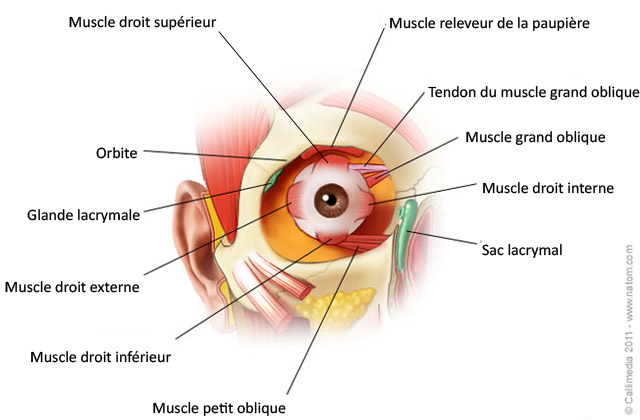
\includegraphics[scale=0.5]{oeil.jpg}
	\caption{Schéma de l'oeil}
	\label{Schéma de l'oeil}
	\end{figure}
	
	\newpage
	
	L’œil d’un être humain adulte est une sphère qui mesure environ 2,5 cm de diamètre, et pèse environ 7 grammes. 
	
	La partie antérieure visible ne représente qu’un sixième de l’œil, le reste est situé dans l’orbite et est entouré de graisse. 
	
    Des structures interviennent dans la protection de l’œil et permettent sont fonctionnement :
    \begin{itemize}
   	\item[$\bullet$] Sourcils : ils permettent de protéger l’œil des gouttes de sueur en provenance du front ainsi que de la lumière,
	\item[$\bullet$] Paupières : les paupières mobiles clignent par reflexe toutes les 3 à 7 secondes, elles peuvent également cligner automatiquement lorsqu’un corps étranger arrive dans l’œil ou un souffle d’air.  Elles protègent l’œil de tous les corps étrangers et permettent également de prévenir la dessiccation (déshydratation de l’œil) car ainsi, les sécrétions telles que le mucus, les larmes, l’huile se répandent à la surface du globe oculaire, son hydratation est alors permanente.  
	\item[$\bullet$] Conjonctive : elle tapisse le blanc de l’œil ainsi que les paupières produisant un mucus lubrifiant.
	\item[$\bullet$] Glande lacrymale : elle sécrète des larmes qui sont répandues sur la surface du globe oculaire grâce aux clignements des yeux, et vont ainsi protéger, nettoyer, humecter et lubrifier la surface de l’œil.
	\end{itemize}	
	
	Chaque globe oculaire est mobile grâce à des muscles fixés dans l’orbite, cavité osseuse du crâne. Ils partent du fond de l’œil et s’attachent sur les côtés du globe oculaire. 
	
    Ces muscles permettent ainsi le mouvement rapide des yeux qui peut aller dans toutes les directions, ils sont au nombre de six, quatre sont droits et deux obliques :        
    \begin{itemize}
    \item[$\bullet$] Le droit supérieur, permet à l’œil de se déplacer vers le haut
	\item[$\bullet$] Le droit inférieur, permet de se déplacer vers le bas
	\item[$\bullet$] Le droit médian (ou interne), permet le déplacement de l’œil vers le nez
	\item[$\bullet$] Le droit latéral (ou externe), permet le déplacement de l’œil vers la tempe
	\item[$\bullet$] L’oblique supérieur (ou grand oblique) Le muscle releveur de la paupière supérieure. 
	\item[$\bullet$] L’oblique inférieur (ou petit oblique) 
	\end{itemize}		
    Trois enveloppes emboitées limitent l’œil humain, la sclérotique, la choroïde et la rétine se prolongeant par le nerf optique :
    \begin{itemize}
	\item[$\bullet$] Sclérotique : c’est une enveloppe opaque et blanche très résistante. Elle devient transparente et forme la cornée à l’avant de l’œil, la face visible. Le rayon de courbure et alors plus petit. Sa netteté va être assurée grâce aux larmes et clignements de l’œil.
	\item[$\bullet$] Choroïde : elle recouvre entièrement la sclérotique et est noire ainsi que vascularisée. Elle devient l’Iris colorée présentant une ouverture à l’avant de l’œil, la pupille.  
	\item[$\bullet$] Rétine ($0,2 \; mm$) : c’est l’enveloppe la plus interne de l’œil, c’est un tissu nerveux grisâtre, mince, collé contre la choroïde et se prolonge par le nerf optique. 
	\end{itemize}	
Avant d’atteindre le fond de l’œil, les rayons lumineux doivent traverser des milieux transparents le contenant :
	\begin{itemize}
	\item[$\bullet$] L’humeur aqueuse a une composition semblable à celle du plasma sanguin et remplit l’espace entre la cornée et le cristallin.
	\item[$\bullet$] Le cristallin, biconvexe, se trouve derrière la pupille et va se déformer grâce à l’action de petits muscles permettant ainsi de modifier sa convexité.
	\item[$\bullet$] L’humeur vitrée est en arrière du cristallin. C’est une substance gélatineuse remplissant l'espace compris entre le cristalline et la rétine.
	\end{itemize}
	
	\begin{figure}[h]
	\begin{center}
	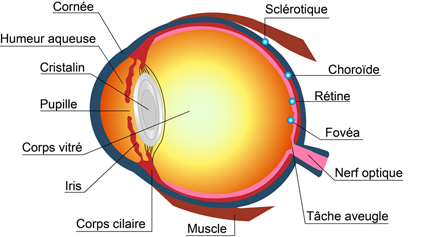
\includegraphics[scale=0.8]{schema_oeil.jpg}
	\end{center}
	\caption{Coupe de l'oeil}
	\label{Coupe de l'oeil}
	\end{figure}
\newpage
	\section{Fonctionnement de l'oeil}
		\subsection{Propagation de la lumière}
		Dans un milieu transparent, homogène et isotrope (c’est-à-dire qui a les mêmes propriétés dans toutes les directions), la lumière se propage en un mouvement rectiligne et uniforme.
		
	Dans le cas où le milieu n’est pas homogène, par exemple lors d’une différence de température, la lumière est déviée : c'est le phénomène de réfraction. Lorsque la lumière change de milieu, nécessairement transparent, elle subit ce phénomène. C’est le cas par exemple de l’eau ou encore l'air. 
	
	Ce sont les lois de Snell-Descartes qui définissent les angles de réfraction. Prenons un exemple : un rayon de lumière, appelé rayon incident, se déplace dans un premier milieu transparent, l'air. Ce rayon traverse ensuite un second milieu transparent, l'eau. Le rayon arrive à la surface de l'eau avec un certain angle par rapport à la normale : c'est \textit{l'angle d'incidence}, noté $i$. Lorsque le rayon traverse l'eau, il est dévié par rapport à la normale. L'angle ici présent est \textit{l'angle de réfraction}, noté $r$, ou parfois $i_{2}$.
	
	Chaque milieu transparent possède un indice de réfraction, noté $n_{milieu}$, différent. Il est pour l'air de $n_{air} = 1,0003$, et pour l'eau de $n_{eau} = 1,333$.
	
	Nous pouvons calculer les angles d'incidence et de réfraction, ou bien les indices de réfraction de différents milieux transparents grâce à la formule :	
	\[
	n_{1} \cdot \sin i = n_{2} \cdot \sin r
	\]	
	La réfraction d’un rayon lumineux, ainsi que la manière dont il est dévié, est donc plus ou moins forte en fonction du milieu qu’il traverse, ainsi qu’en fonction de l’angle d’incidence.
	
	\begin{SCfigure}[][h]
	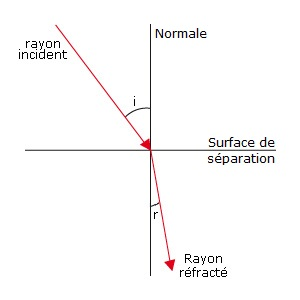
\includegraphics[scale=0.6]{refraction.jpg}
	\caption{Schéma de la réfraction}
	\end{SCfigure}	
	
	 En plus du phénomène de réfraction, la lumière subit un phénomène de dispersion. Par exemple, si un faisceau de lumière blanche est dirigé vers une surface plane d'un bloc de verre, elle est décomposée lors de sa réfraction : le spectre de la lumière blanche apparaît.
	 
	 \begin{figure}[h]
	 \begin{center}
	 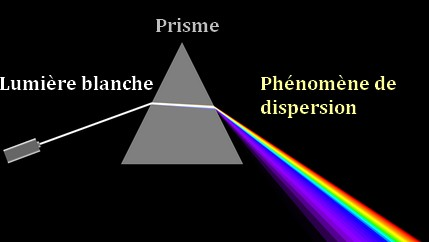
\includegraphics[scale=0.73]{dispersion.jpg} 
	 \end{center}
	 \caption{Schéma de la dispersion}
	 \label{Schéma de la dispersion}
	 \end{figure}	 
	 
	 La dispersion est à l’origine des arc-en-ciel : la lumière passe à travers des gouttes d’eau, qui dispersent la lumière, et font apparaître le spectre de la lumière blanche. 

		\subsection{Formation d'une image}
		L’œil est un organe, disposant d’une rétine qui tapisse son fond, dont le but est de former une image à partir de rayons de lumière puis de l’envoyer au cerveau afin qu’il la traite. En plus d’être capable de détecter la lumière, l’œil doit aussi pouvoir détecter sa direction. 
		
	Tout d’abord, nous allons nous intéresser à la formation d’une image dans un milieu quelconque.
	
	Lorsqu’un objet est éclairé par une source lumineuse, des rayons de lumière se forment. Lorsque l’on intercale une lentille convergente entre ces rayons, nous constatons qu’ils convergent en un point.
	
	\begin{figure}[h]
	\begin{center}
	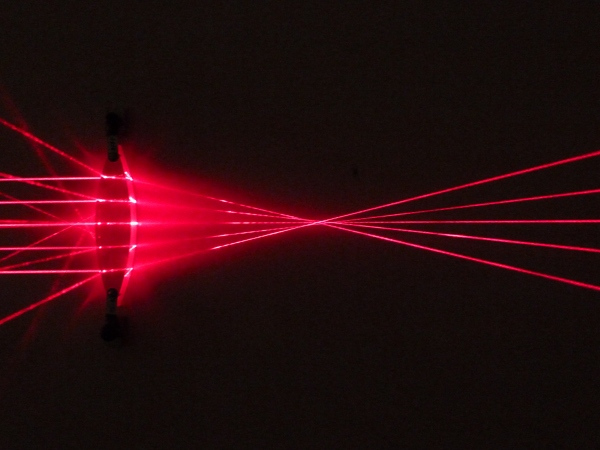
\includegraphics[scale=0.3]{lentille_convergente.jpg}
	\end{center}
	\caption{Lentille convergente}
	\label{Lentille convergente}
	\end{figure}
		
	Si l’on positionne un écran après le foyer image, on constate l’apparition d’une image dessus : c’est l’image formée à partir de l’objet. En fonction de l’endroit où se situe l’objet par rapport à la lentille, l’image sera plus ou moins grande, et plus ou moins éloignée de la lentille. Aussi, elle est toujours renversée. 
	
	\begin{figure}[h]
	\begin{center}
	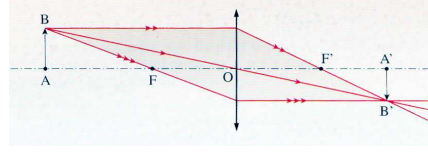
\includegraphics[scale=0.9]{formation_image.png}
	\end{center}
	\caption{Construction d'un objet}
	\label{Construction d'un objet}
	\end{figure}
		
		La formation d’une image suit trois règles :
		\begin{itemize}
		\item[$\bullet$] Si l’objet est situé à l’infini, l’image se forme au foyer,
		\item[$\bullet$] Si l’objet est situé à la distance focale, l’image est située à l’infini,
		\item[$\bullet$] Si la distance entre la lentille et l’objet est supérieure à la distance focale, l’image est située après la lentille, et est renversée.
		\end{itemize}
		
	Dans le cas d’une loupe, l’objet est situé après le foyer objet, l’image est dans le bon sens, et se forme avant l’objet : c’est une image virtuelle.

\newpage
		\subsection{L'oeil}
		L’œil est composé d’un cristallin, qui peut être assimilé à une lentille convergente. Lorsque les rayons lumineux provenant d’un objet éclairé y pénètrent, ils convergent donc en un point. L’image formée à partir de l’objet est une image inversée.
		
		Lorsqu’un objet est éclairé, nous pouvons le voir. En effet, les rayons lumineux qui en proviennent passent à travers l’iris, et rentrent dans l’œil. Ils subissent une réfraction lorsqu’ils traversent l’humeur vitrée et aqueuse, et peuvent donc former l’image renversée sur la rétine.
		
	\begin{figure}[h]
	\begin{center}
	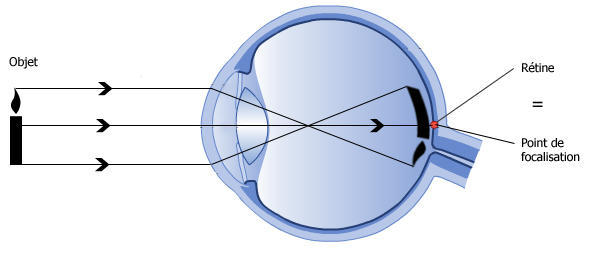
\includegraphics[scale=0.2]{rayons_lumineux.jpg}
	\end{center}
	\caption{Rayons lumineux}
	\label{Rayons lumineux}
	\end{figure}
		
	L’œil dispose d’un système d’accommodation. Il est sur ce point assimilable à un appareil photo, qui possède une fonction de mise au point. Pour l’œil, le cristallin se déforme plus ou moins. Par exemple, plus un objet est proche, et plus le cristallin va se courber. Par conséquent, sa distance focale diminue, et sa vergence augmente. 

	L’œil est un organe pouvant posséder des défauts.

\newpage
	\subsubsection{La myopie}
	L’œil est trop convergent, et les images se forment avant la rétine. Le positionnement d’une lentille divergente devant l’œil peut corriger ce problème.	Elle est le plus souvent due à un œil trop long. Ainsi lorsqu’on fixe un objet éloigné, son image se forme donc en avant de la rétine, la vision de loin est alors floue. Cependant la vision de pré est nette. Ce défaut de l’œil permet ainsi de lire sans lunettes, mais plus elle est développée, plus le texte doit être rapproché. 
	
	\begin{figure}[h]
	\begin{center}
	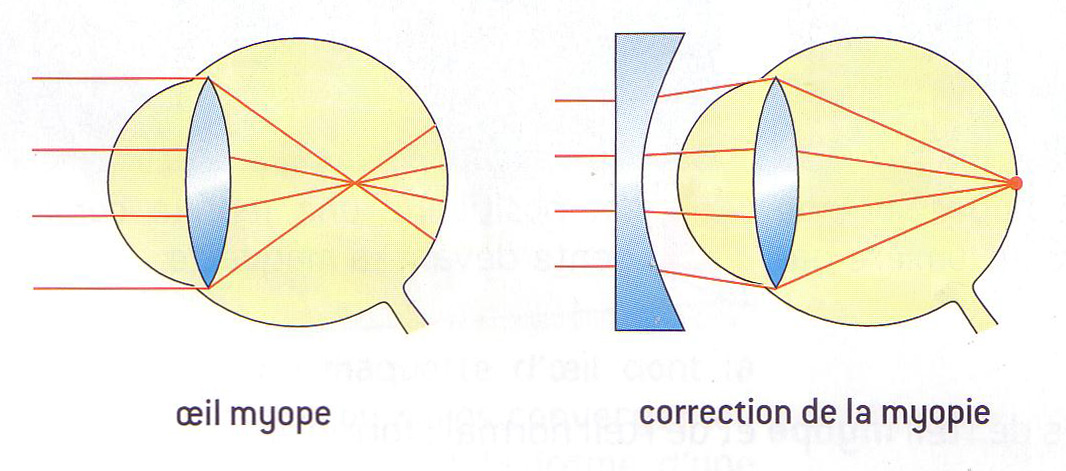
\includegraphics{myopie.jpg}
	\end{center}
	\caption{Myopie et sa correction}
	\label{Myopie et sa correction}
	\end{figure}
	
	\subsubsection{L'hypermétropie}
	C’est le contraire de la myopie, l’œil n’est pas assez convergent, et donc les images se forment après la rétine. Il faut cette fois-ci placer une lentille convergente devant l’œil.	C’est l’inverse de la myopie, l’œil dans ce cas est généralement trop court, l’image d’un objet éloigné se forme alors en arrière de la rétine. La personne observera ainsi des difficultés à lire de près cependant elle voit relativement bien de loin et n’est alors pas gênée dans ce cas la. 
	
	\begin{figure}[h]
	\begin{center}
	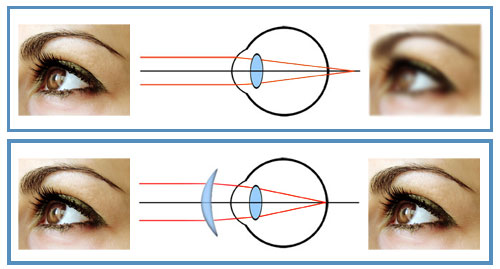
\includegraphics[scale=0.5]{hypermetropie.jpg}
	\end{center}
	\caption{Hypermétropie et sa correction}
	\label{Hypermétropie et sa correction}
	\end{figure}
	
	\subsubsection{La presbytie}
	C’est un défaut de l’œil qui apparaît en général chez les personnes âgées. En effet, le cristallin est « fatigué », il ne peut plus accommoder. De ce fait, les images de près se forment derrière la rétine. Il faut cette fois également porter des lunettes convergentes. C’est un phénomène habituel de vieillissement de l’œil. C’est la diminution naturelle de la capacité d’accommodation du cristallin notamment lors de la lecture. Pour pouvoir voir de près, le cristallin doit se bomber rapidement afin de restituer une image nette au cerveau qu’elle que soit la distance qui le sépare de l’objet observé, c’est l’accommodation. Elle permet la mise au point de l’œil comme le ferait un appareil photo avec l’autofocus. Le cristallin vieillit et perd de son élasticité en fonction de l’âge, l’accommodation diminue elle aussi, elle est alors importante chez l’enfant est va diminuer plus la personne vieillit.   
	
	\begin{figure}[h]
	\begin{center}
	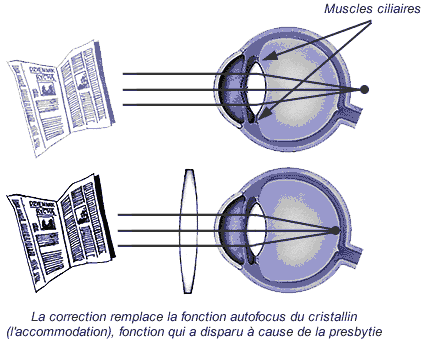
\includegraphics[scale=0.7]{presbytie.png}
	\end{center}
	\caption{Presbytie et sa correction}
	\label{Presbytie et sa correction}
	\end{figure}
	
	\subsubsection{L'astigmatisme}
	C’est un défaut de la composition de l’humeur aqueuse et/ou de l’humeur vitrée. Les rayons qui les traversent ne forment plus un point lumineux sur la rétine, mais une tache de dimension et de formes variées. C’est une anomalie de courbure de la cornée qui est irrégulière, elle est ovale au lieu d’être ronde. Les rayons lumineux se focalisent alors en des points différents, à la fois en arrière et en avant de la rétine. L’image perçue est alors déformée, par exemple l’œil astigmate ne verra nettes que les lignes horizontales ou verticales, la vision est brouillée, floue et imprécise. Il y a des confusions de lettres proches comme le M le N et le H, le 8 et le 0. L’image d’un point n’est pas un point mais une droite. 
	
	La vision n’est jamais excellente sans être vraiment mauvaise, que ce soit de près ou de loin. 
	
	\begin{figure}[h]
	\begin{center}	
	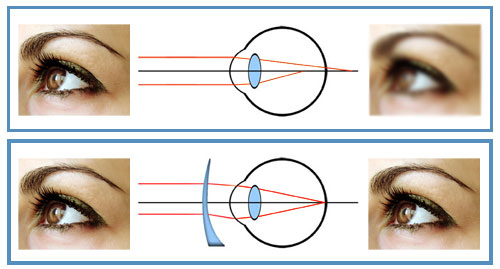
\includegraphics[scale=0.5]{astigmatisme3.jpg}
	\end{center}
	\caption{Astigmatisme et sa correction}
	\label{Astigmatisme et sa correction}
	\end{figure}
	
	\newpage
	
	\subsection{La rétine}
	
	La rétine est un tissu nerveux, c’est un prolongement du cerveau. Elle est composée de cellules photosensibles, c'est-à-dire sensibles à la lumière. Ces cellules peuvent être de deux types : des cônes et des bâtonnets. 
	
	Les cônes détectent les couleurs, ils sont donc sensibles soit au vert, au rouge ou au bleu. C’est ainsi que l’œil va pouvoir détecter toutes les couleurs, grâce à la combinaison de ces cônes. 
	
	Les bâtonnets, quant à eux, ne peuvent détecter que le noir et le blanc, mais sont sensibles aux faibles luminosités : c’est ce qui fait qu’on dispose d’une vision nocturne, et donc que nous n’y voyons pas de couleurs.
	
	Il existe une zone située au centre de la rétine, la fovéa, dont chacune des cellules est reliée à une seule cellule nerveuse. C’est cette zone qui est à l’origine de l’acuité visuelle (le fait de voir nettement un petit objet lointain), car chacune des cellules la composant captera un point lumineux différent de celui capté par les autres cellules.
	
	\begin{figure}[h]
	\begin{center}
	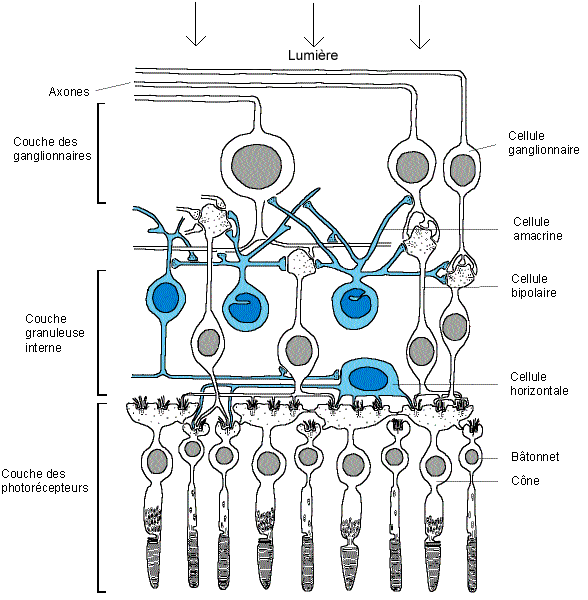
\includegraphics[scale=0.5]{retine.png}
	\end{center}
	\caption{Composition de la rétine}
	\label{Composition de la rétine}
	\end{figure}
	
	Nous voyons dans ce schéma que la lumière entre dans la rétine, puis traverse différentes couches de cellules, pour arriver enfin à celle des photorécepteurs. Les cônes et les bâtonnets contiennent un pigment visuel, qui absorbe certaines radiations du spectre de la lumière blanche. Ce pigment permet de transformer le flux de photons en message nerveux. Celui-ci fait ensuite le chemin inverse de celui de la lumière, jusqu'aux axones, qui mènent au nerf optique, donc au cerveau.
	
	La présence de ce nerf optique dans la rétine est à l'origine de la \textit{tâche aveugle}. En effet, cette zone est dépourvue de cellules photosensibles, et ne peut donc pas capter la lumière.
	
	Après avoir découvert le fonctionnement de l’œil, nous allons nous intéresser à celui du cerveau dans le cadre de la vue.

\newpage
	\section{Fonctionnement du cerveau dans le cadre de la vue}
	\sectionmark{Le cerveau}
	Le cerveau est l’organe central du corps humain. C’est lui qui contrôle le fonctionnement des autres organes. Dans le cadre de la vue, il est capable de recevoir un message nerveux provenant de l’œil, plus précisément de la rétine, par le nerf optique, qui contient une image captée par l’œil, et de l’interpréter.
	
	C'est par le sens de la vue que nous percevons la lumière, les formes et les couleurs, que nous apprécions les détails des objets, leur distance et leur relief.
	
	Les informations visuelles recueillies par l'œil sont transformées en messages nerveux au niveau de la rétine, puis transmit par les nerfs optiques jusqu'au cerveau. C'est alors le cortex visuel qui analyse le stimulus reçu, élabore la perception visuelle et répond de façon appropriée.
	
	Comment une image est-elle transmise par l’œil au cerveau ? Comment celui-ci l’interprète ?

		\subsection{Transmission de l'image}
		Tout d'abord il faut savoir que  l'œil est mobile grâce à des muscles fixés dans l'orbite. C'est un système optique qui permet la formation d'une image réelle, et surtout  renversée par rapport à l'objet regardé.  
	
	L'intérieur des globes oculaires est rempli de différents milieux transparents jouant le rôle d'une lentille, qui permettent donc la formation d'une image au fond de l'œil. Il s'agit de l'humeur aqueuse, du cristallin et de l'humeur vitrée.
	
	Entre l'iris et la cornée se trouve un espace rempli d'humeur aqueuse, un fluide semblable à l'eau.
	
	Ensuite derrière l'iris se trouve le cristallin, une lentille transparente biconvexe (offrant deux faces arrondies opposées) qui permet de faire la « mise au point » pour des objets rapprochés.
	
	Comment l'image parvient-elle au cerveau ?
	
	L'absorption de lumière par les pigments photosensibles des cônes et des bâtonnets modifie leurs propriétés électriques et conduit à la naissance d'un message nerveux. En effet, si la stimulation visuelle est suffisante, un message nerveux, constitué d'une succession de signaux électriques, est généré dans les fibres du nerf optique. Une variation de l'intensité du stimulus visuel se traduit alors par une variation de la fréquence des signaux électriques.
	
	Les messages nerveux visuels générés par la rétine sont acheminés par les nerfs optiques jusqu'au cerveau.
	
	Le nerf optique de l'œil droit et celui de l'œil gauche se croisent au niveau du chiasma optique. À cet endroit, la moitié des fibres de chacun des nerfs optiques s'entrecroisent et passent dans l'hémisphère opposé. Les autres fibres rejoignent directement le lobe occipital du cerveau, où se trouvent les centres d'interprétation de la vision. Ainsi, chaque hémisphère reçoit des informations visuelles issues des deux yeux.
		
	\begin{figure}[h]
	\begin{center}
	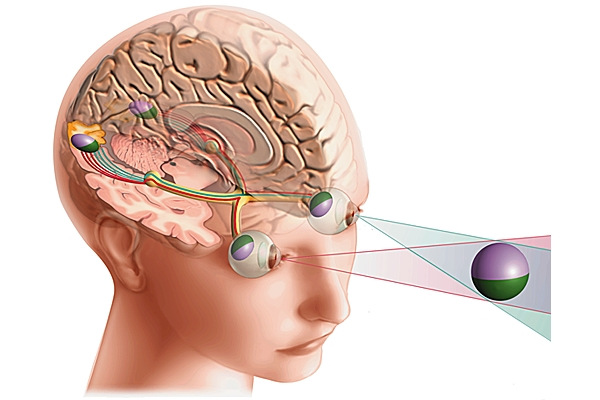
\includegraphics[scale=0.7]{deux_yeux.jpg}		
	\end{center}
	\caption{Vision d'une image à travers les deux yeux}
	\label{Vision d'une image à travers les deux yeux}
	\end{figure}
	
	Il existe une zone de relais, située entre le chiasma optique et le cortex visuel, dans laquelle toutes les fibres des nerfs optiques sont en connexion synaptique avec d'autres neurones qui conduisent les messages jusqu'au cortex visuel. La transmission du message nerveux se fait alors par l'intermédiaire de substances chimiques, les neurotransmetteurs.
	
	Ainsi, certaines substances hallucinogènes, en se fixant sur les récepteurs de ces neurotransmetteurs, modifient la perception visuelle. 
	Les substances hallucinogènes proviennent de certains éléments végétaux, soit les plantes.  Elles peuvent également être synthétisées en laboratoires, elles ont alors un autre nom, celui de drogues psychédéliques, ce qui signifie une ouverture d’esprit sur une autre perception de soi et du monde.
	
	Ces dernières ont des effets constatés sur le corps humain à savoir dans le cas de notre recherche sur l’œil. 
Les substances hallucinogènes vont provoquer chez l’usager une perception inhabituelle de son monde intérieur et extérieur. Ces dernières peuvent être minimes ou bien importantes, elles peuvent parfois dépasser ces stades et aller jusqu'à l’hallucination. 

	Ces substances exercent leur effet au niveau du système nerveux, elles vont perturber la transmission du message nerveux dans les synapses. En effet, elles ont une structure moléculaire en partie semblable à celle du neurotransmetteur naturel qui a pour but de transmettre le message nerveux. Ainsi ces substances peuvent se fixer sur les récepteurs, à la place de ces neurotransmetteurs. 
	
	Certaines substances vont avoir la capacité de renforcer l’action de ce dernier, on est alors victime d’une exagération de la transmission du message nerveux. D’autres à l’inverse diminuent l’action du neurotransmetteur et limitent ainsi la transmission du message nerveux. La vision va alors être modifiée différemment pour chaque individu ; devenant d’une beauté indescriptible chez les uns ou à l’inverse entraînant terreur angoisse et peur chez les autres. Une même personne peut être confrontée aux deux types de modifications visuelles. 
	
	L’exemple le plus connu est celui du LSD (de l’allemand « Lyserg Saüre Diäthylamid »), une substance chimique dérivée de composants qui sont présents naturellement dans certains champignons. Cette substance hallucinogène est connue pour provoquer des visions particulièrement colorées. 
	
	D’autres substances altèrent la perception sensorielle des indivis. L’alcool quant à lui diminue le champ visuel ; l’appréciation des distances et modifiée. 
	
	Le cannabis perturbe lui aussi la vision, la perception des sons est exacerbée, poussée à l’extrême. 

\newpage
		\subsection{Interprétation de l'image}
		Différentes régions du cerveau sont impliquées dans le processus de la vision : le cortex visuel primaire mais aussi différentes aires cérébrales spécialisées.
		
	Après avoir franchi la zone de relais, la plupart des messages nerveux visuels arrivent dans une aire située à l'arrière du cortex occipital de chacun des deux hémisphères. Ces deux aires cérébrales forment le cortex visuel primaire. Chacune d'entre elles reçoit des informations provenant des deux yeux. Ainsi, toute lésion située dans cette zone provoque une cécité plus ou moins prononcée. Parallèlement, certaines informations visuelles arrivent directement dans différentes aires visuelles spécialisées dans le traitement de la couleur, des formes ou encore des mouvements.
	
	Ainsi, toutes les informations concernant une image sont traitées en parallèle. Leur intégration et les échanges entre l'ensemble de ces aires permettent ensuite d'avoir une perception globale et unifiée.
	
	Les gènes interviennent dans l'organisation et la structure du cortex visuel et sont, par conséquent, impliqués dans la perception visuelle. Ces structures sont similaires chez tous les individus, ce qui donne initialement à chacun les mêmes potentialités visuelles.
	
	À condition d'être stimulées, les capacités visuelles se développent entre 0 et 10 ans, en même temps que le cerveau.
	
	En outre, l'environnement et l'expérience individuelle ont une influence sur les structures corticales mises en jeu dans la vision.
	
	Le cortex est divisé en plusieurs aires corticales spécifiques (V1, V2, V3, V4 et V5). Il n'est pas nécessaire d'expliquer la fonction de ces aires corticales car cela ne nous intéresse pas, or on peut ajouter que l'aire corticale V4 est chargée du traitement des formes et des couleurs.

\chapter{Comment le cerveau peut-il être trompé ?}
\chaptermark{L'expérience}
	\section{Présentation de notre expérience}
	L'expérience que nous allons vous présenter aujourd'hui en avant première est apparemment bluffante. Action vidéo.
	Avez vous vu le changement de sens des flèches?? 
	
	Qu'en pensez vous?? pour vous est-ce une hallucination , un phénomène optique, une illusion d'optique effet d'optique mirage.
Avouons-le, ce tour de magie n'en est pas un, ce n'est pas non plus une véritable illusion optique. 
Même si cette expérience est impressionnante, elle est par ailleurs scientifiquement explicable. En effet ce tour de magie est  un effet optique .  C'est un événement observable, due à l'interaction entre la lumiere et la matiere le plus souvent soumise a un facteur environnementale ici en l'occurrence le verre et l'eau.
	\section{Explication de l'expérience : comment l'a-t-on construite et pourquoi est-ce un effet d'optique ?}
	\sectionmark{Explications}
	\subsection{Au préalable}
	Notre expérience met en œuvre le principe de réfraction. Nous disposons donc d'un verre, de l'eau, ainsi que d'un objet bicolore : en l'occurrence un T-Shirt blanc à gauche et noir à droite. Lorsque nous réalisons l'expérience, nous voyons donc que les couleurs du T-Shirt sont inversées. La lumière provenant de l'objet passe à travers le verre d'eau, il change donc de milieu. Ce changement de milieu conduit les rayons lumineux à être déviés et donc à l'image d'apparaître autrement. 
	
	Cependant, il faut faire attention au fait que les rayons traversent également le verre, qui est un autre milieu transparent. 
	
	Prenons l'exemple d'une lame de verre de forme parallélépipédique d'une certaine épaisseur, que l'on va noter $e$. Lorsque le rayon incident arrive à la surface de cette lame avec un angle d'incidence $i$, il subit le phénomène de réfraction et est par conséquent dévié. Il possède donc un angle de réfraction $r$. Cependant, ce même rayons sort ensuite du verre. Il change donc une fois de plus de milieu : une autre réfraction se produit. Étant donné que la normale ($N$) à la première couche de verre est parallèle à la seconde ($N'$), le rayon incident sort de la lame de verre avec un rayon incident de valeur $r$, et est dévié avec un angle de réfraction de valeur $i$. 
	
	En conséquence, lorsque le rayon traverse une lame de verre, il est simplement légèrement décalé par rapport à son point d'arrivée. Il garde le même angle d'incidence. Ceci est valable pour n'importe quelle épaisseur de verre. 
	
	\begin{figure}[h]
	\begin{center}
	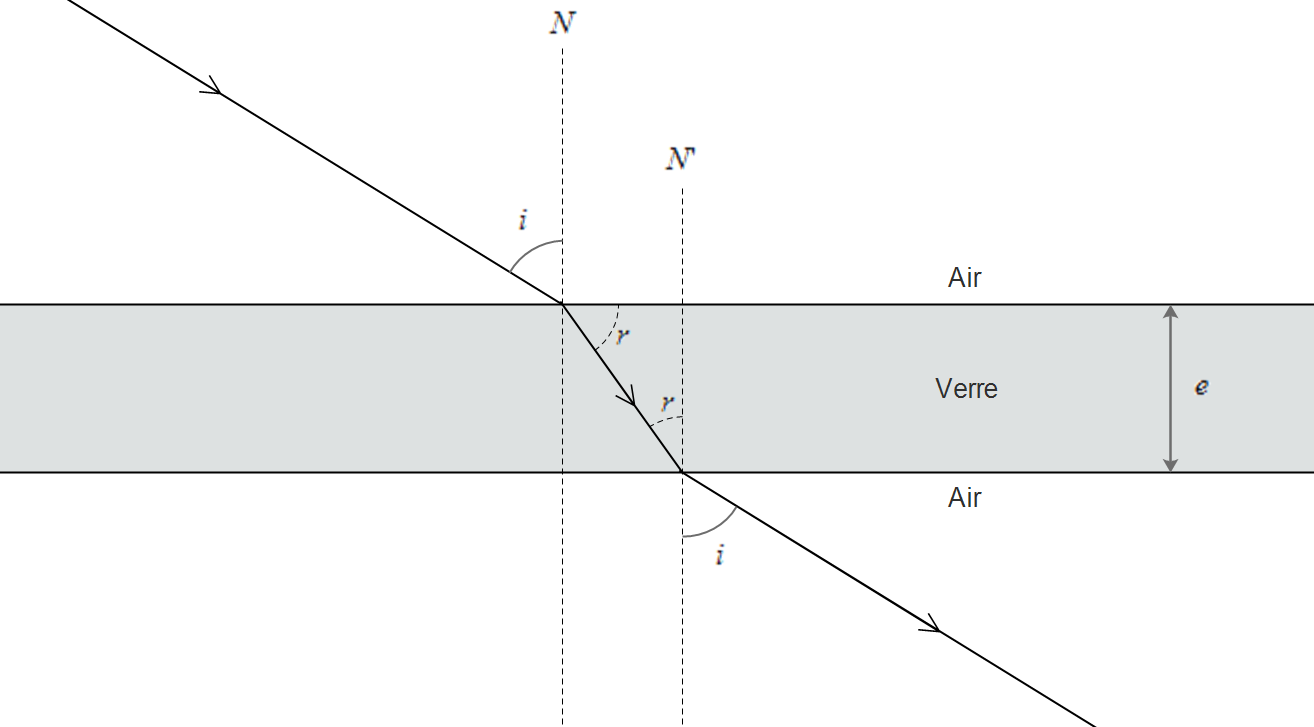
\includegraphics[scale=0.5]{refraction-theorie1.png}
	\end{center}
	\caption{Réfraction air-verre-air (verre droit)}
	\label{Réfraction air-verre-air (verre droit)}
	\end{figure}
	
	\newpage
	
	Cependant, dans notre exemple, nous n'utilisons pas une lame de verre parallélépipédique mais courbée. Le principe est ici le même. Le rayon est réfracté de la même manière. Néanmoins, comme le verre est courbé, la normale correspondant à la seconde réfraction ($N'$) n'est pas parallèle à celle de la première ($N$). Ainsi, l'angle d'incidence du premier rayon réfracté n'est pas égal à son angle de réfraction. La différence entre les valeurs de $r$ et de ce nouvel angle $r'$ est cependant très faible pour un verre classique (donc d'assez faible épaisseur). 
	
	\begin{figure}[h]
	\begin{center}
	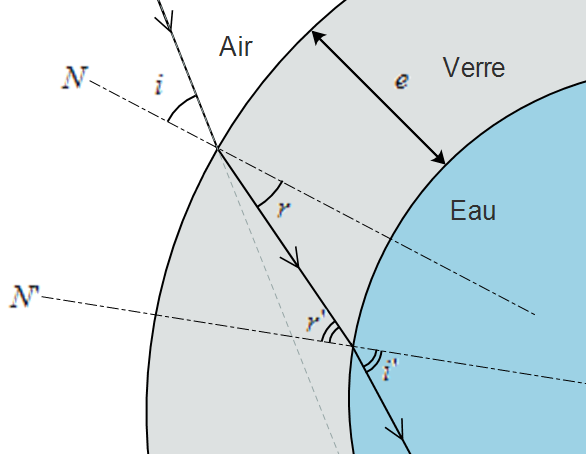
\includegraphics[scale=0.5]{refraction-theorie2.png}
	\end{center}
	\caption{Réfraction air-verre-eau (verre courbé)}
	\label{Réfraction air-verre-air (verre droit)}
	\end{figure}
	
	Comme $r$ est différent de $r'$, le rayon de lumière n'est plus réfracté de la la même manière, et le nouvel angle d'incidence $i'$ n'est plus égal à $i$. Donc dans le cas de notre verre, la lumière est non seulement décalée par rapport à son origine, mais également légèrement déviée. Cependant, comme ces paramètres sont très faibles, nous n'en tiendront pas compte pour la suite de l'explication.
	
	\newpage
	\subsection{Explications}
	
	Nous assimilons donc notre verre d'eau à un simple cylindre d'eau (sans bords). Chaque rayon de lumière issu de l'objet va rencontrer le cylindre, et donc être dévié. Ensuite, le rayons change à nouveau de milieu en sortant du cylindre : il passe de l'eau à l'air. La réfraction fait qu'il se retrouve dans le même sens que le rayon au début, mais à l'opposé. Ainsi, la partie blanche du T-Shirt, initialement à gauche, se retrouve à droite, et la partie noire à gauche. Voici un schéma de ce qu'il s'est produit (\textit{pour des raisons de clarté, nous avons dessiné la partie blanche du T-Shirt en rouge}) :
	
	\begin{figure}[h]
	\begin{center}
	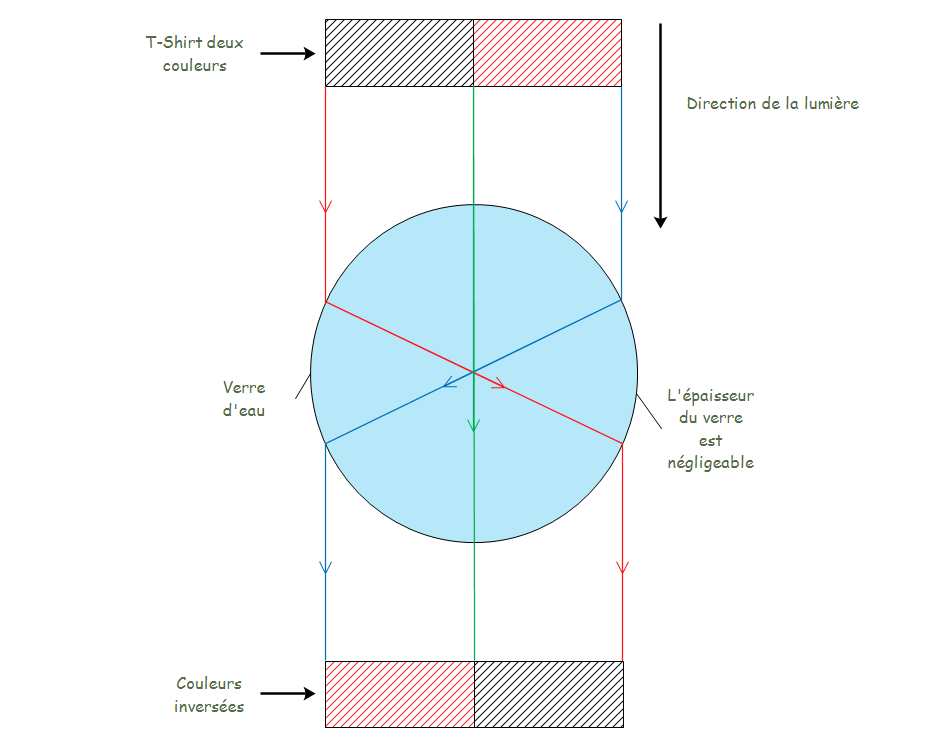
\includegraphics[scale=0.7]{refraction-experience.png}
	\end{center}
	\caption{Notre expérience schématisée}
	\label{Notre expérience schématisée}
	\end{figure}
	
\chapter{Autres exemples d'illusion}
	\section{Différence entre illusion et effet d'optique}
	\section{Mirages}
	En été, lorsqu’on regarde au loin une route, on a l’impression de voir des flaques d’eau au sol. Celles-ci, disparaissent quand on se rapproche, c’est un mirage. 
	
	Le mot « mirage » vient du latin \textit{miror}, \textit{mirari} qui signifie s’étonner, voir <<avec étonnement>>. C’est tout comme notre propre illusion que nous vous avons présenté un phénomène optique. Les mirages sont dus à la déviation des faisceaux lumineux par des superpositions de couches d’air de températures différentes.  
A cause de la déviation de ces rayons, on ne voit pas l’objet à son réel emplacement, l’image perçue est alors souvent déformée. 
	
	Le mirage n’est pas une illusion d’optique, qui est une déformation d’une image à cause d’une interprétation erronée du cerveau, on peut le photographier, ce n’est donc pas une hallucination, on parlera simplement de phénomène optique. 
	
	On regroupe les mirages en trois catégories, les mirages supérieurs, les mirages inférieurs et le \textit{Fata Morgana}, les plus complexes, composés de plusieurs images superposées les unes aux autres. 

\paragraph{Principe d'un mirage :}
	L’indice de réfaction de l’air peut évoluer grâce à la température, la pression atmosphérique ou encore l’humidité ou la composition de l’air. 

	Les couches d’air froid sont par exemples plus denses que les couches d’air chaud. 
L’indice de réfaction des couches d’air froid est alors plus fort, ce dernier évoluant en fonction de la pression et de la température. 

	Une superposition de couches d’air de température de plus en plus importantes ou à l’inverse de couches de plus en plus froides crée un gradient de température et de pression et donc d’indice pour l’air. 

	Pour un état normal, dans l’atmosphère, une colonne d’air a un gradient de température d’environ $-1\times 10^{-2} ~^{o}C.m^{-1}$, provoquant dès cette température faible des phénomènes de « réfraction terrestre » permettant dès lors la déformation ou la vision de certains objets non visibles normalement, tels les bateaux à l’horizon. 
	
	Pour que l’on parle véritablement de mirage, le gradient doit avoir une température d’au moins $2$, voir $4 ~^{o}C.m^{-1}$. 


\paragraph{Mirage inférieur :}
	Ce mirage également appelé « mirage chaud » est causé par le réchauffement des couches basses de l’air ; on l’aperçoit souvent l’été au niveau des routes chauffées par le soleil ou encore dans les zones désertiques. 
Dans ce cas la, l’air proche du sol peut avoir des températures bien supérieures à celles des couches les plus élevées (parfois plus de $10 ~^{o}C$ de différence).

	Les rayons lumineux vont ainsi être très courbés au niveau de cette partie près du sol. Reposant sur un échauffement de l’air au niveau du sol assez important, les images perçues seront déformées à cause de turbulences ; les routes ne donnent pas une réflexion parfaite du ciel mais une image approximative, telles des flaques d’eau. 

\paragraph{Mirage supérieur :}
	Aussi appelé « mirage froid » ce mirage apparaît lorsque l’air à la surface du sol est plus froid que celui en hauteur.  A certains endroits où la surface du sol est extrêmement froide telle que les banquises, les sols gelés ou encore les mers froides, l’air est refroidi au niveau du sol, car par phénomène de convection, l’air chaud monte en altitude.Apparaît alors des couches d’air plus froid appelées couches d’inversion.  L’image observée au niveau du sol ou près de celui-ci sera ainsi au dessus de l’objet réel, elle peut être déformée ou encore inversée.
	
	Dans ce type de mirage, la trajectoire des rayons lumineux issus de l’objet va être ascendante et concave, cela apparaît lorsque les rayons suivent la courbe de la Terre, c’est ainsi qu’un objet situé sous l’horizon peut être perçu au dessus. 

\paragraph{Fata Morgana et FataBromosa :}
	Dans certaines situations, il arrive qu’un mirage inférieur et un mirage supérieur se combinent ; il apparaît ainsi à l’observateur une image irréelle au paysage lointain. 
	Il s’agit d’un mirage peu stable donnant plusieurs images différentes, déformés et superposées de l’objet de ce dernier. 
	Il est particulièrement observable dans le détroit de Messine, situé dans la mer Méditerranée séparant la péninsule italienne de l’île de Sicile. 
	
	La Fata Morgana est due à une superposition de couches d’inversion et de couches d’air chaud avec des gradients plus ou moins forts. Ainsi le rivage lointain est élevé au-dessus de l’horizon par un phénomène de mirage supérieur, dû aux couches d’inversion. D’autres parties sont élargies et déformées a cause d’une partie d’air plus chaud, une partie des rayons est ainsi ramenée vers le sol.  Le paysage à l’horizon se trouve alors complètement déformé, des tours ou immeubles sont allongés par les couches d’inversion, des plateaux sont élargis et superposés grâce aux couches d’air plus chaud. 
	
	La FataBromosa, aussi appelée \textit{Brumée de fée} est provoquée de la même façon, mais l’image crée se trouve plutôt aplatie car les rayons réfractés ne sont que dans certaines zones uniquement, ainsi des parties sombres ou d’autres très lumineuses sont perçues,  on peut alors observer un contraste de brouillard brillant à l’horizon. 

Ces deux effets peuvent eux-mêmes être combinés, il est courant que des FataBromosa soient incluses dans une Fata Morgana. 

	\section{Stéréogrammes}
	Les stéréogrammes sont des images en 3 dimensions où sont dissimulées des formes. Ils apparaissent sous forme d’une texture abstraite, mais avec un agencement particulier, qui permet de faire apparaître la forme recherchée.
	
	Il existe manières de les voir : il faut placer son visage le plus près possible de l’image. En effet, lorsqu’on regarde une image ou un objet, nos yeux sont focalisés sur un point situé derrière l’image. L’image reçue par chaque œil est différente, mais le cerveau les interprète comme si c’étaient les mêmes. Le cerveau est capable de reconstituer le relief caché dans le stéréogramme, mais seulement si on se focalise dessus. Se placer très près de l’image fait que les yeux ne peuvent plus faire le point, ils regardent alors le vide. Ensuite, il faut reculer doucement, toujours en gardant le même type de vision. 
	
	Voici un exemple de stéréogramme :
	
\part*{Annexes}
\listoffigures
\end{document}
